
%*******************************************
\section{Approach for Our Anti-Phishing Education App}
%*******************************************
\label{s:approach}
This chapter presents our final approach for the Anti-Phishing Education App.
 In the following sections we will elaborate on the app design in detail.

%===========================================
\subsection{App Design}
%===========================================
\label{s:app_design}
We have decided to divide our education app into two main parts.
 The first part of the education app is intended to increase the user awareness.
 The second part of the app then covers the actual educational part.
 The following enumeration summarizes the functions of our twofold app structure.

\begin{enumerate}
	\item \textbf{Awareness Part} The first part of the education app is intended to increase the user awareness regarding how easy it is to spoof e-mails and mislead users with such fake messages.
 This part is supposed to motivate the user to do something to counter the danger of the Internet, in this particular case, against phishing.

\begin{enumerate}
		\item \textbf{Receive Fake E-Mail} We want to illustrate to the user how easy it is to spoof the ``from'' field of an e-mail as well as the content of this e-mail.
 For this purpose the user has to send a fake e-mail with an arbitrary sender address of his choice to himself.
 The user will also have the option to type in a free text.
 Upon submitting the form the user will receive an e-mail with the e-mail address he had indicated as sender.
 The free text will also be part of the received e-mail.
 We believe that the user will be very surprised about how easy even he himself could send a fake e-mail.
 The user will learn that he cannot fully trust the ``from'' field and the content of the e-mails he is receiving.

		\item \textbf{Linktext Unequal Target URL} The awareness part of the app is also supposed to show the user that he cannot trust the texts of a link he is clicking on.
 To illustrate this, the user is asked to click on a link with the text ``https://www.
google.
de/''. Clicking on this link, the user will expect to land on the Google website, what will not happen.
 In fact, the user is linked back to our app, where he is told that link texts are not trustful as well.
 
	\item \textbf{Fake Website} Finally, the user is told that creating a copy of a website is also very easy.
 He is told that a reliable way to decide whether a website is a fake or not is to analyze the URL of the website he is visiting.
 He is also told that this app focuses on exactly this.

\end{enumerate}
	\item \textbf{Educational Part} The second part of the app covers the actual educational part.
 Here, the user is learning about various spoofing techniques of the attacker.

\begin{enumerate}
	\item \textbf{Information Material} The second part of the app is divided into levels of increasing difficulty.
 Here the user is first taught how to access and analyze the URL of the web browser.
 Subsequently, the user learns about the general structure of a URL.
 This is done in a very simplified way, so that even unexperienced users can follow.
 In particular, the user is told how to find the second- and top-level domain of a URL.
 In all succeeding levels the user is introduced to various URL spoofing techniques of a phisher.
 The learning content of each level can be consulted in~Section~\autoref{s:knowledgetransferperlevel}.
		\item \textbf{Exercise to Information Material} After every introductory material in each level an exercise section is followed.
 For the ``access and analyze URL part'', for example, the user is forwarded to a website.
 There he has to apply all important steps he has learnt in the introductory part.
 After successful completion of the tasks the user is linked back to the app.
 For the ``find second- and top-level domain'' information material the user gets a couple of valid URLs of which he has to identify the second- and top-level domains.
 All subsequent level exercises are structured as follows: the user is presented a URL.
 He has to decide whether the presented URL is a phish or a valid URL.
 If the URL is a phish, and the user has correctly identified the phish, the user has to show the second- and top-level domain.
 Only if the user correctly identifies the second- and top-level domain he receives the points for this URL, otherwise the answer to this URL is considered wrong, because we assume that the user has just guessed in this case.

		\item \textbf{Repeat 2.a and 2.b With Increasing Difficulty} There is an increase of difficulty in each level.
 That is to say, in each level it gets more difficult to distinguish phishing URLs from valid ones, cf.
~Section~\autoref{s:knowledgetransferperlevel}.
\end{enumerate}
\end{enumerate}

The next section deals with the concrete rules of the game.

%===========================================
\subsection{Gamification}
%===========================================
As we pointed out we decided on designing the app as game.
This is mainly because we think that this makes it more interesting for the users and raises the possiblity that we reach more users.
In most modern games we see the following elements which we all implemented:
\begin{description}
\item[Levels] Most games have some kind of level system.
This has multiple purposes.
First it is important for the player to get a feeling for the process he makes in the game.
It also provides the user with fixed points in the game where he can restart or pause and play on later.
To us it gives the ability to structure the game in a repeating cycle that the user learns.
This way if the user plays multiple levels in a row he can skip the repeat parts easily but if he has paused he can read it.
The details of the leveling Strategy can be found in Section \autoref{a:mail}
\end{description}
User motivation

\subsubsection{Leveling}

\begin{description}
	\item[Show Leaderboard Rate]
	\item[Show Leaderboard Total]
	\item[Lives]
	\item[Levels]
	\item[Leveling]
\end{description}


%===========================================
\subsection{Game Rules}
%===========================================
The educational part of the app which is followed by the awareness part is divided into several levels.
 In each level the user is provided with specific informational material.
 After the information material is consulted by the user, he has to finish the according exercise.
The first  and second information materials (introduction 2 and level 1) and exercises that the user receives differ from the ones of the other levels. Here, the users obtain basic knowledge in order to bring them to the same knowledge level for the actual game.
 
\begin{description}[leftmargin=0cm]
	\item[Basic Knowledge]  The first information material and task of the user deals with accessing the address bar of a webbrowser and viewing its URL completetely.
 To prove that the user has understood how to access the address bar and view the URL he has to do the following: When the user is forwarded to the website to solve the task he has to scroll up to the top of the website to make the generally hidden address bar visible.
 Afterwards, he has to provide us the information we request about the URL in the address bar.
 This will show that he has in fact viewed the whole URL.
 After successful completion the user is linked back to the app and level 1 is started.
 From this level on, the user has three lives upon start of each level.
 In level 1 he has to identify the ``Who-Section'' (second- and top-level domain) of a URL.
 He has to tap the according part of the displayed URL.
 In this level wrong answers result in losing points and losing a live.
 In order not to frustrate the user he cannot get less than 0 points.
 When the user has no more lives left he has to restart the level.
 With every correct answer the user gains points.
	\item[Start of Actual Game]  In level 2 we start introducing URL spoofing techniques and the user has to decide whether a given URL is a phishing URL or a valid one.
 Here also, the user can lose and win points as well as lose lives.
 Here again, if the user has no more lives left he has to restart the level.
 The following Figure~\autoref{fig:lose_points_life} illustrates the game flow and consequences of wrong and correct answers from level 2 and upwards.
 If the user has correctly decided that a phishing URL is a phish, he has to show us the ``Who-Section'' to prove that he has understood the concept.
 In all other cases the user is directly shown the result of his answer.
 In summary, the user looses points for any wrong answer, but he does not lose a life for every wrong answer.
 We have decided that rejecting valid URLs is not as severe as accepting phishing URLs.
 For this reason the punishment for accepting a phishing URL is more severe than the punishment for rejecting a valid URL.
 All in all, the user loses points and a live in the following cases: the user has falsely accepted a phishing URL or the user has correctly rejected a phishing URL, but could not show us the ``Who-Section''. In all other cases the user cannot lose lives, but only points.
\end{description}

The following section deals with our leveling strategy.

\begin{figure}[hHtbp]
\centering
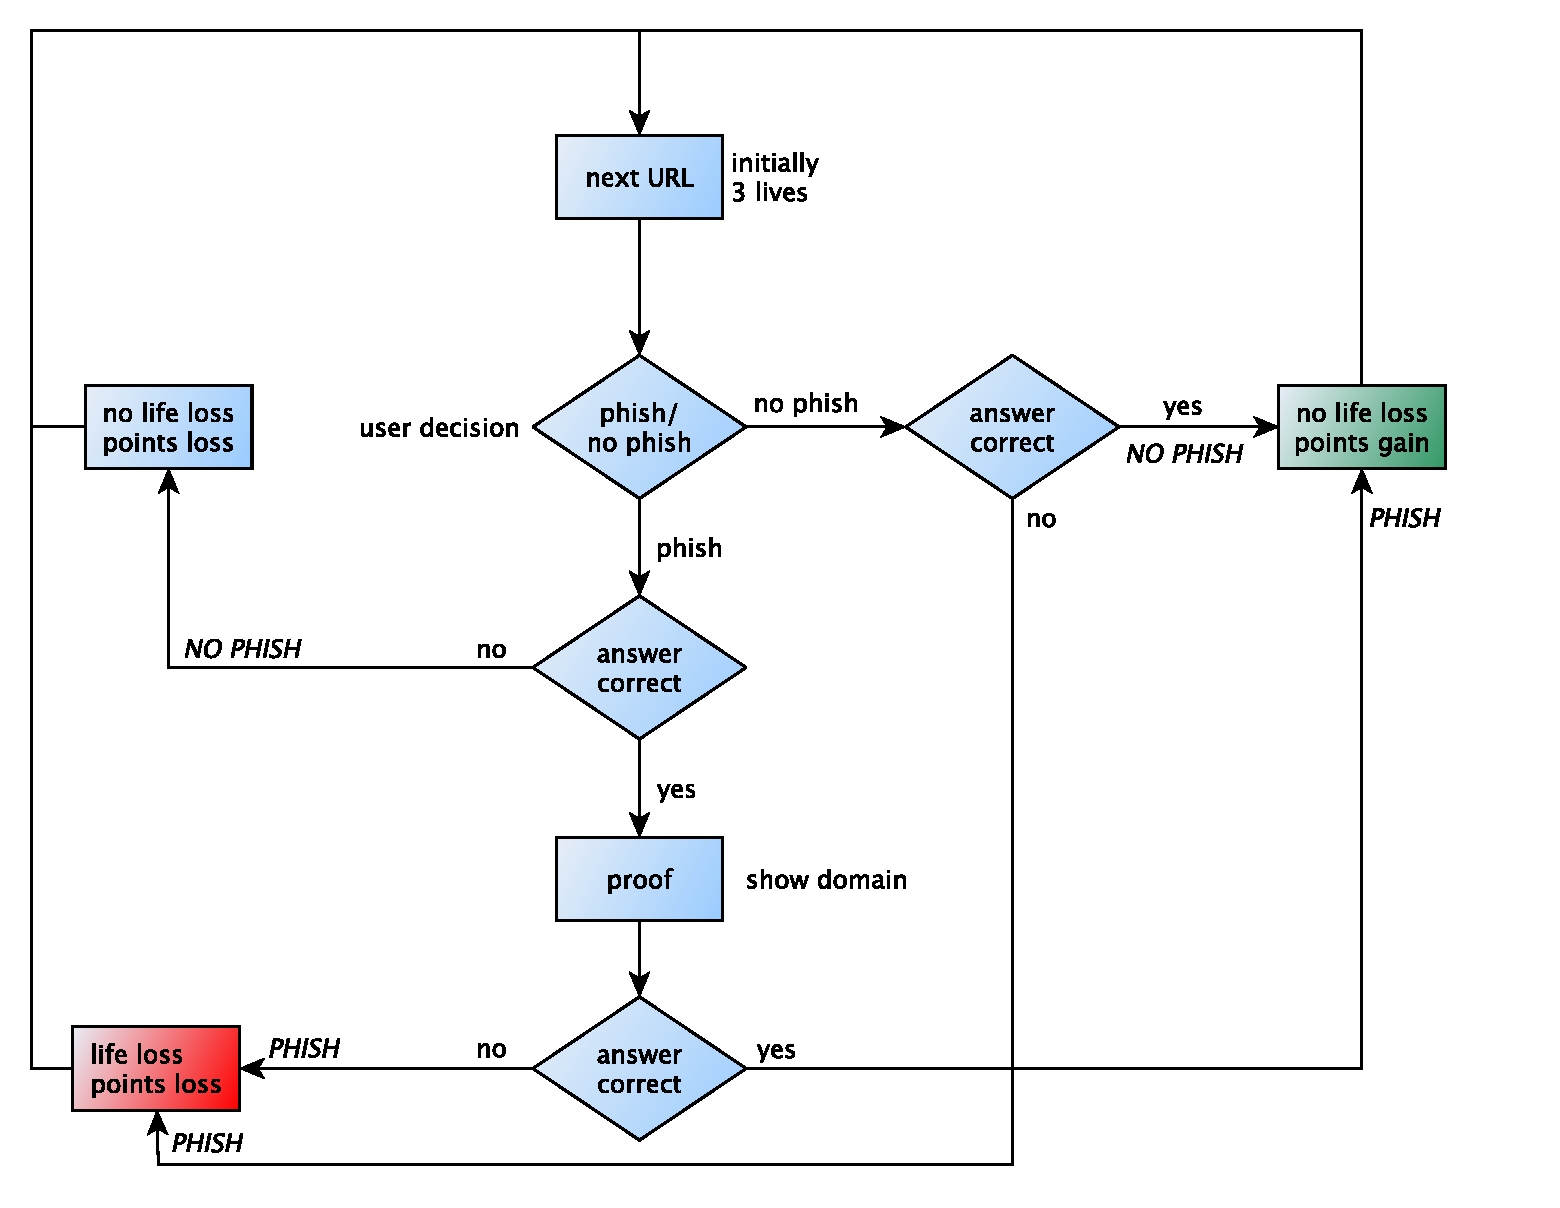
\includegraphics[width=1.0\textwidth]{graphix/lose_win_points.pdf}
\caption{Losing points and lives in the game}
\label{fig:lose_points_life}
\end{figure}
%===========================================
\subsection{Leveling Strategy}
\label{s:leveling}
%===========================================
During the app development we have tried out several leveling strategies.
 This section is intended to introduce the leveling strategies we have considered for the app.


\begin{description}[leftmargin=0cm]
	\item[Leveling Based on Achieved Points] Our very first leveling strategy was based on the achieved points per level.
 Each level the user had to achieve at least 100 points to pass the current level and unlock the next one.
 This approach had a major drawback.
 The fact that achieving a minimum of points to pass the level resulted in very similar points for everybody finishing a level.
 That is to say, everybody who has finished level x, has approximately the same points, which in turn would have meant that the comparison between single users would not be meaningful as it would only differ very slightly.
 Additionally, with this strategy, users might replay early levels which are easier and gain the same amount of points as users playing later levels.
 This might result in users playing early levels repeatedly get more points than users playing later and difficult levels.

	\item[Leveling Based on Detected Phishes] The previously described leveling strategy had the deficit of comparability among the users.
 However, we consider comparability very important  since it serves as an incentive for the user to play better or play on.
 For this reason we overthought our strategy and decided that passing a level should not depend on the points a user receives.
 It rather should depend on the number of phishes the user was able to detect during a level.
 That is to say, among the shown URLs in every level there is a certain amount of phishes the user has to detect in order to pass the level.
 With this approach however, there is still the possibility for a user to repeat early, and thus easy, levels and possibly gain more points than users playing later, and thus more difficult, levels.
 To prohibit this, in increasing levels the users gains and loses increasing points accordingly.
 In this way, a user repeating early levels is not able to catch up other users of higher levels.
 This strategy solved the problems of our first strategy, however it also brought a new one.
 The strategy of passing the level when a certain amount of phishes are detected has the following flaw: always rejecting a URL will eventually result in passing the level (if the user also correctly identifies the ``Who-Section'' when required). The user will not gain a lot of points with this strategy, however he will eventually win, which is suboptimal for a game.
  
	\item[Leveling Based on Correct Answers] To solve the problem of our second leveling approach we have extended the leveling passing to correct answers.
 Instead of detecting a certain amount of phishes per level, the user has to give correct answers to a predefined amount of phishing URLs as well as a predefined amount of valid URLs in order to pass the level.
 Only and only if the user has answered the predefined number of valid and phishing URLs the level is completed.
 To additionally incentivize the users we have included three lives per level.
 The lives are supposed to prevent a user playing eternally, without ever passing the current level.
 When the user loses all of his lives, cf.
~Figure~\autoref{fig:lose_points_life}, this is an indication that he did not understand what the level is about.
 Consequently, he has to restart the level by being forwarded to the introductory part of the current level.
 This is our final leveling strategy for the app.

\end{description}


%===========================================
\subsection{Teaching Goals Per Level}
%===========================================
\label{s:knowledgetransferperlevel}
This section summarizes the learning objectives of each level.
 Note that we generally do not use technical terms like URL, domain, subdomain, protocol or the like. Figure~\autoref{fig:level_teaching_goals} illustrates and exemplifies the level flow of our app.


\begin{description}[leftmargin=0cm]
	\item[Introduction 1] This part is the awareness part described in Section~\autoref{s:app_design}. Here, the user learns how easy e-mail spoofing is.
 Additionally, the user is informed about the simplicity of setting up fake websites and that he should not trust the texts of the links he is clicking on.

	\item[Introduction 2] In this part the user is explained how he can access the URL of a web browser and how exactly he has to look at the whole URL.
 In particular, the user is told that he has to scroll up the whole website to make the generally hidden address bar re-appear.
 Then he has to tap the text field of the address bar and scroll to the start of the URL.
 At the end of the exercise for this the user is told that he always has to analyze the URL like this, because all other displayed URLs or links might be fake too.

	\item[Level 1] The actual game starts with level 1, where the user learns about the structure of a URL.
 First of all, the user gets an overview of the single components of a URL.
 To make the comprehension of these components easier to understand we used an analogy which is summarized in Figure~\autoref{fig:url_components} with an example URL.
 We told the user that he has to imagine that the website he is visiting is his dialog partner.
 The user is told that the section between ``http(s)://'' and the third slash ``/'', i.
e.
 the hostname, reveals information about his dialog partner.
 In particular, we explain that he has to read this part from right to left.
 The top-level and second-level domain is introduced as ``Who-Section'' (company + location of company), from which the user knows who he is actually talking to.
 All succeeding parts in this area are to be considered as ``departments'' of the company of ther user's dialog partner.
 The protocol part is introduced as ``Security Level'' of the dialog with the partner and the path part of a URL, i.
e.
 the part after the third slash ``/'', is introduced as the topic of the conversation with the dialog partner.
 When marking parts of a URL we consistently used the according colour of Figure~\autoref{fig:url_components}. The main objective of the level 1 exercise is to be able to identify the second- and top-level domain of a URL.

	\item[Level 2] With level two we start introducing the spoofing tricks of a phisher.
 We considered the subdomain attack, cf.
~Section~\autoref{s:url_categories}, as a good starting point to introduce the phisher as the user has just learnt about the importance of the ``Who-Section'' (top-level and second-level domain) in level 1.
	\item[Level 3] In level 3 the user is first told what an IP address is.
 To facilitate the comprehensibility, we used the analogy of house addresses.
 The user is explained that like addressing our houses with street names and numbers, computers in the Internet are addressed by so called IP addresses.
 The IP address itself is defined as a 4-place sequence of numbers, separated by dots.
 Finally, the user is warned against URLs with IP addresses in the host part.

	\item[Level 4] In this level we deal with nonsense in the second-level domain, cf.
~Section~\autoref{s:url_categories}.
	\item[Level 5] In this level we deal with second-level domain names which sound trustworthy, but are in fact unrelated to the company name, cf.
~Section~\autoref{s:url_categories}.
	\item[Level 6] Here misleading and deceiving names in the second-level domain of a URL are covered.
 This includes typos, scrambled letters or other similar and deceptive names in the second-level domain, cf.
~Section~\autoref{s:url_categories}.
	\item[Level 7] In this level we focus on homographic attacks, where the user is able to visually distinguish a fake second-level domain from the original one, cf.
~Section~\autoref{s:url_categories}.
	\item[Level 8] In this level the user is introduced to an attack where the brand name of the visited website or even the whole legitimate URL is placed in the path of a fake URL, cf.
~Section~\autoref{s:url_categories}.
	\item[Level 9] Here we introduce the difference between the usage of http:// and https://. In particular, the user is told that the usage of https:// means that his conversation with the website is encrypted and that the dialog partner indicated in the ``Who-Section'' is authenticated.
 As an analogy we say that the https:// represents a higher security level.
 This means, the conversation cannot be eavesdroppbed by a third party and the dialog partner indictated in the ``Who-Section'' has proved his identity to a trusted third party.
 With http:// this security level is not established.

	\item[Level 10] This level does not include an exercise.
 It mainly serves as a section with some important additional input for the user.
 Specifically, we tell the user two things: First, we explain to him that he might encounter URLs which actually look very phishy.
 In such a case, we suggest him to directly contact the company and ask for the authenticity of the specific website.
 Furthermore, we introduce extended validation certificates.
 We provide the user with a link to further information to this subject.

\end{description}

\begin{figure}[hHtbp]
\centering
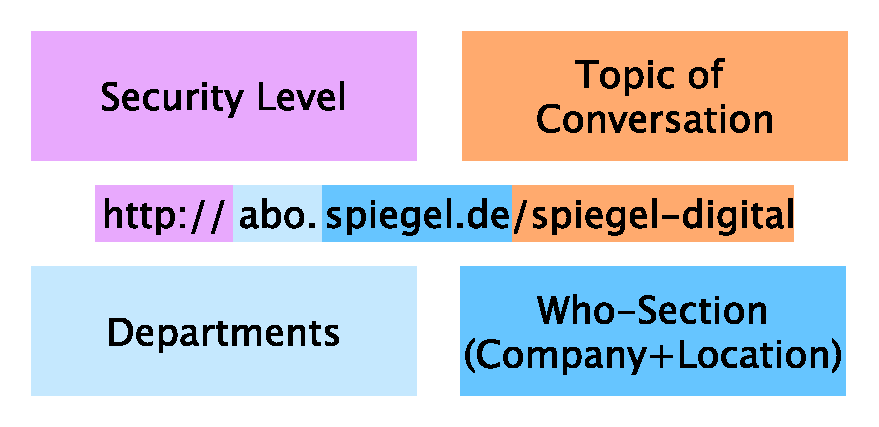
\includegraphics[width=0.56\textwidth]{graphix/url_components.pdf}
\caption{URL components that are communicated to the user}
\label{fig:url_components}
\end{figure}

\begin{figure}[hHtbp]
\centering
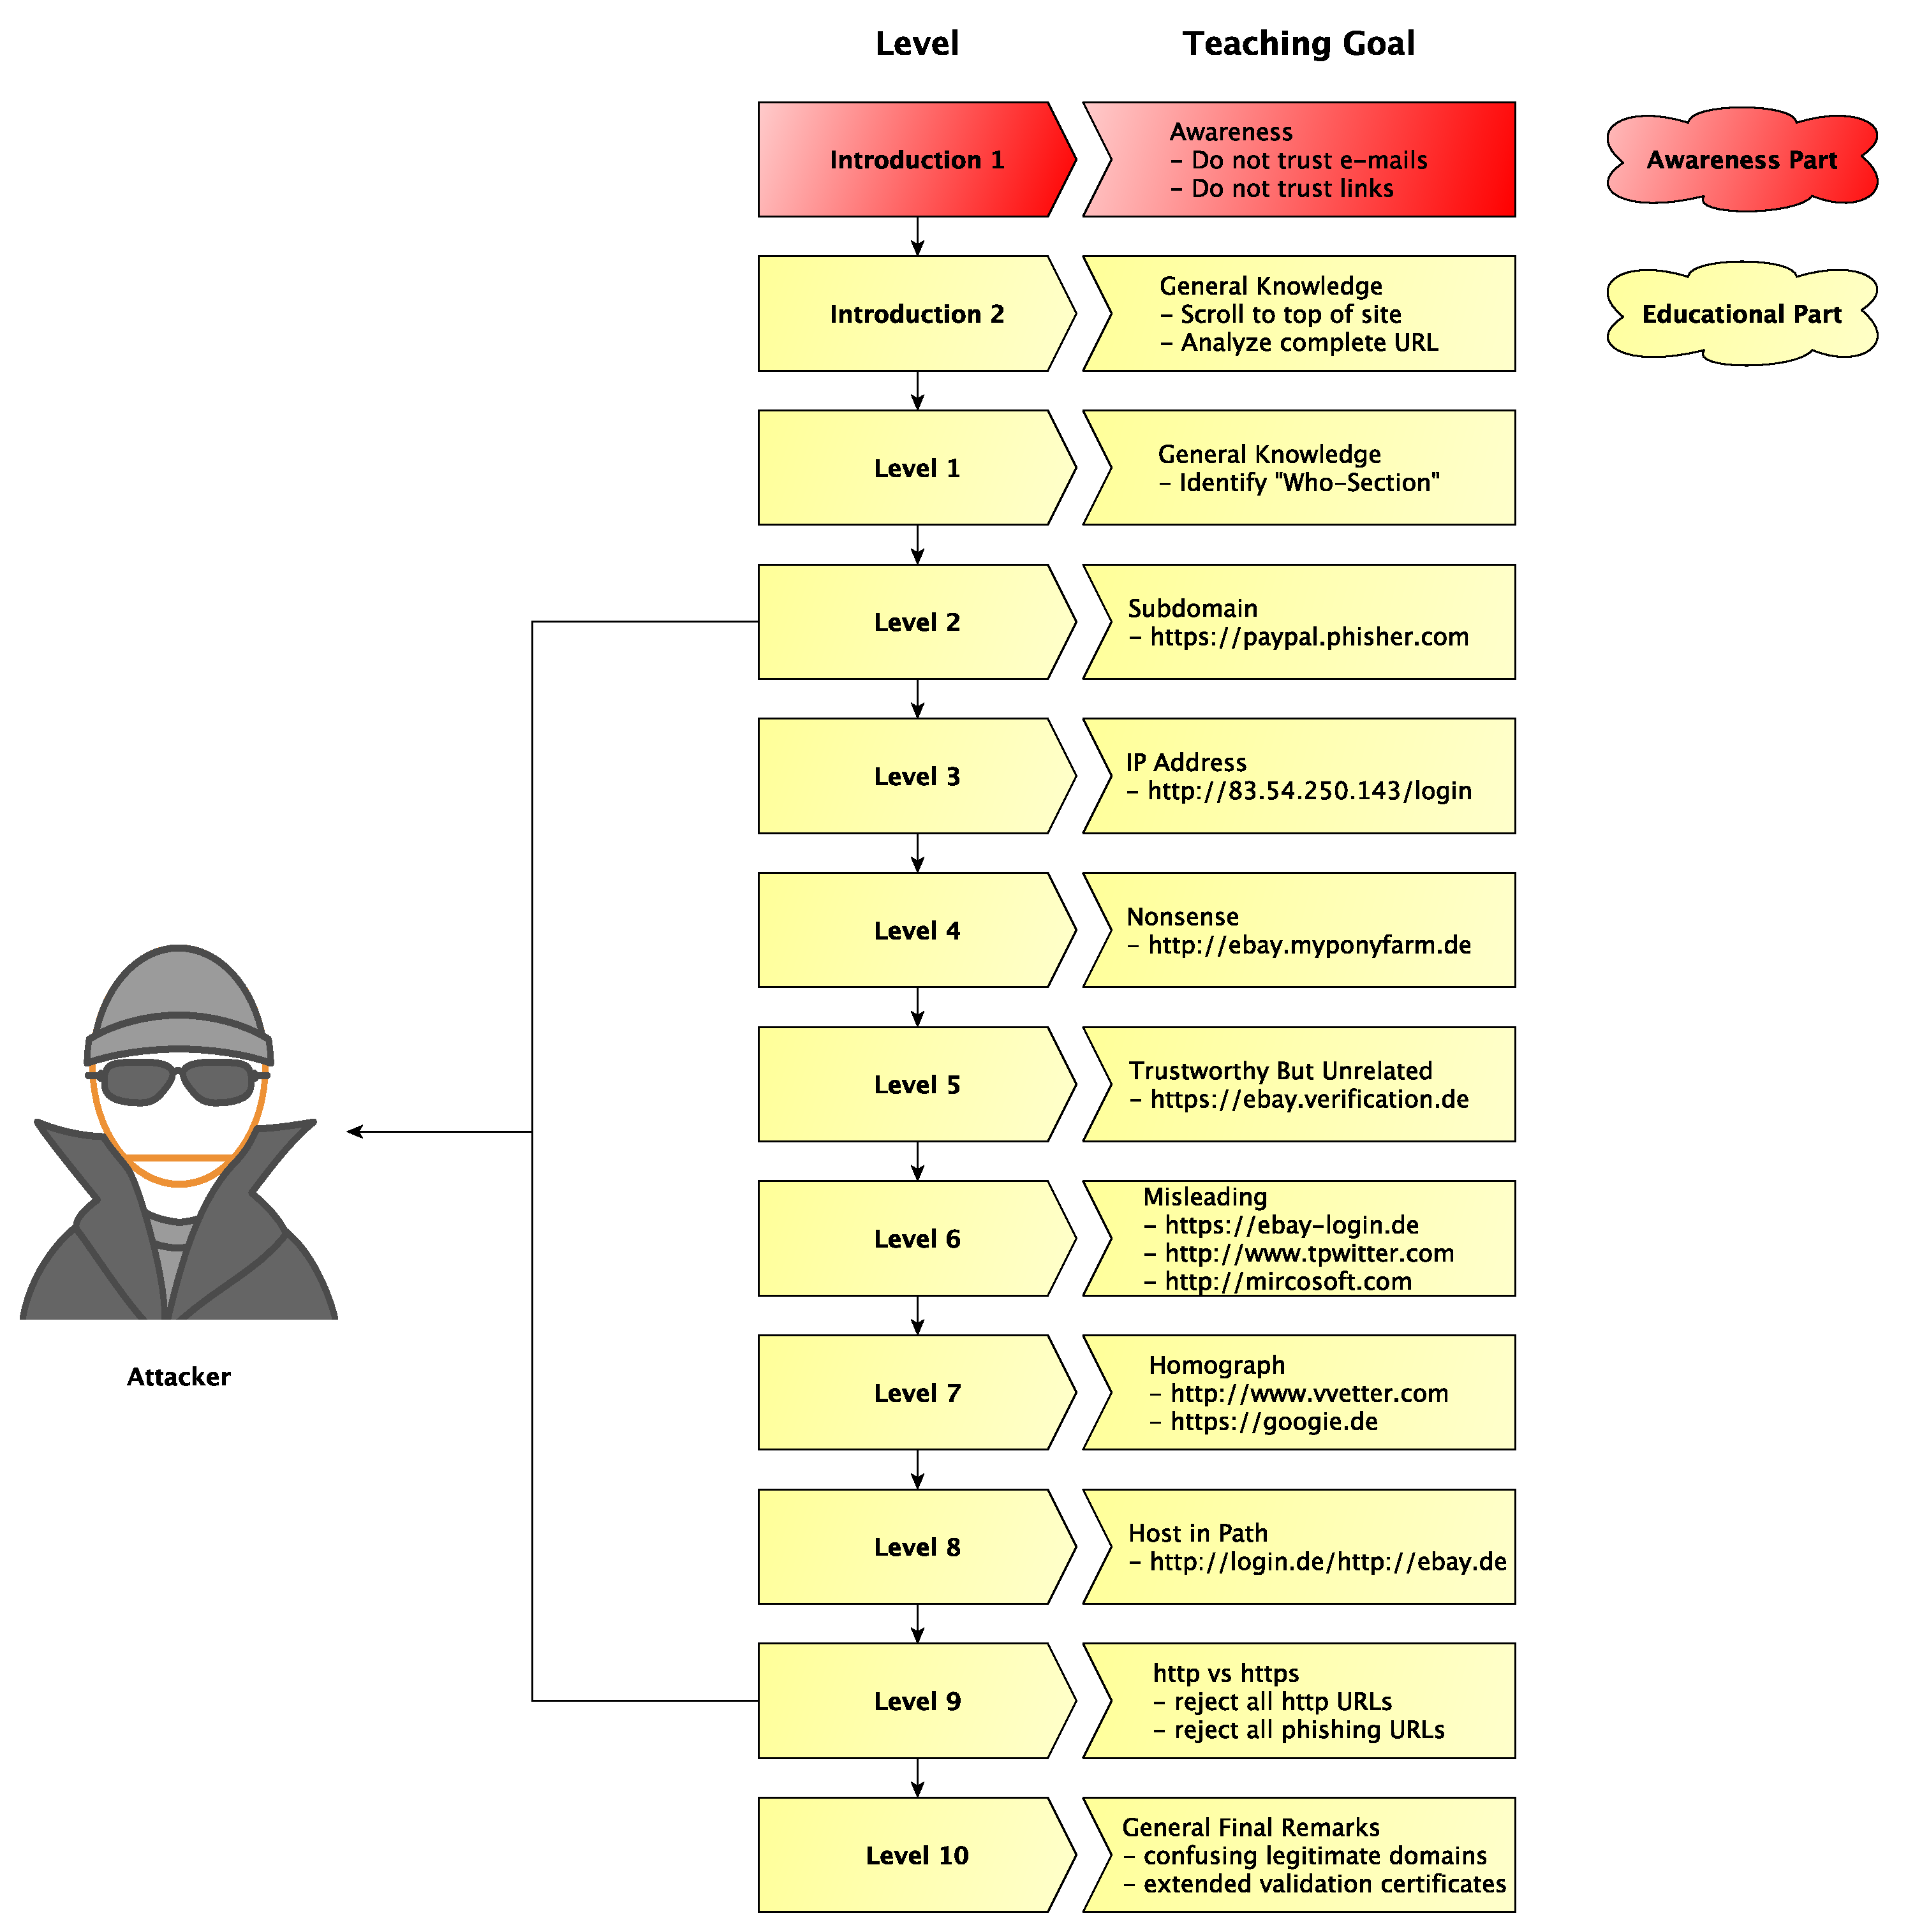
\includegraphics[width=1.0\textwidth]{graphix/level_teaching_goals.pdf}
\caption{Teaching goals of the app}
\label{fig:level_teaching_goals}
\end{figure}


%===========================================
\subsection{Use of Learning Principles and Game Techniques}
%===========================================
Our app is a learning game which purposes to introduce information on the topic of phishing and how to detect it.
With the app we want to improve understanding for this topic and help users be less vulnerable for falling for such attacks in future.
This section deals with the principles of learning and game techniques which are reflected in our app design.
In fact, the laws of learning and game techniques have a strong connection which is the reason why games work for learning purposes~\cite{murphy2011games}.
%--------------------------------------------------------------------------
\subsubsection{Principles of Learning}
%--------------------------------------------------------------------------
\label{s:learning_principles}
Edward Thorndike introduced the first three principles of learning: readiness, exercise and effect~\cite{thorndike1932fundamentals, murphy2011games, handbook2008us}. 
Later the principles of learning were further extended by: primacy, intensity and recency~\cite{murphy2011games, handbook2008us}.
These principles outline how people learn and which conditions improve their process of learning.
In the following we will briefly introduce the meaning of these principles~\cite{murphy2011games} and explain how they are reflected in our app.

\begin{description}[leftmargin=0cm]
	\item[Readiness] The principle of readiness claims that physical, mental as well as emotional preparedness is an important prerequisite for a better learning performance. 
It also states that motivation is crucial for effective learning. 
First of all, students must want to learn something, otherwise any additional motivational efforts will be of no use. 
In order to make students want to learn something it is relevant for them to see a clear reason for learning, i.e. the perceived value of the material is ultimately related to their motivation. 
Finally, the principle of readiness says that best learning performances are achieved in combination with good physical health.
The physical and health conditions of our app users are beyond our control.
For this reason this is an aspect which cannot be reflected in our app.
The app is targeted at users who are willing to learn something about phishing. 
Consequently, there is already some kind of motivation in our app users.
In order to increase this motivation we present clear reasons why the user should continue to play our app.
This is happening in the awareness part, where the user is told what exactly phishing is, how easy it is to phish users, spoof e-mail senders and content, spoof links as well as create exact copies of legitimate websites, cf.~Section~\autoref{s:app_design}.
	\item[Exercise] The use of exercise is composed of two important parts: 
First, training and repetition help increase learning. 
Second, feedback is crucial for good learning performance.
For best learning results, these two parts must be applied together.
In a nutshell, the learning connection is strengthened by practice, and weakend by disuse~\cite{handbook2008us}.
After finishing the awareness part, we start with the user education and provide exercises for all of our learning goals (except for the last level), cf.~Section~\autoref{s:knowledgetransferperlevel}.
The learning content is also permanently repeated. 
For example, in the introduction 2, cf.~Section~\autoref{s:knowledgetransferperlevel} the user learns to scroll up to make the address bar re-appear and analyze the URL by right and left scrolling it. 
The scrolling of the URL is present in levels 2-9.
Also, the user has to identify the Who-Section in level 1. 
In addition, the user has to show the Who-Section every time he has detected a phishing URL correctly.
Finally, every introduced attack of each level n will appear in level n+1 at least once. 
That is to say, as soon as the user gets to know a new attack, he will keep seeing this attack in the succeeding levels.
Our app also provides direct feedback to the users' actions. 
In case of correct answers, the user is rewarded with gained points, with a smiley and a small text that he has done well.
When the user has made a mistake he is punished with losing points, possible life loss and a sad smiley. Also, told that the answer was wrong, why it was wrong and additionally he gets a reminder text on the applied URL spoofing attack he was not able to recognize.
To sum it up, we let our app users practice what we taught them and make use of repetitions in combination with direct feedback.
	\item[Effect] A student who associates his learning with positive feelings will learn more and better than another student who connects his learning with negative feelings. 
For example, a student who is unsuccessful with initial learning material will associate his experience with unpleasantness, frustration, anger and/or confusion, while a student with early success will have strong positive feelings and thus will be more motivated to have more success in future.
Therefore, enabling particularly early success and maintaining student motivation with positive feedback and comments is crucial.
In our app early success is easy to achieve, since we start with easy tasks and obvious attacks which get increasingly difficult in higher levels.
When the user has given a correct answer he is rewarded with a big smiley face as well as points. 
Also, the user is shown a medal every time he finishes a level.
These aspects of the app are intended to increase the users' positive feelings and keep him motivated to go on. 
However, some improvement of positive comments might be worth considering.
Currently, the positive texts for a correctly answered text, for finishing a level and icons do not differ. 
It might be more engaging if such texts and icons differ from time to time in order to increase the positive emotions of the user. 
For example, texts telling the user that he has done well might slightly vary (for instance, according to the degree of difficulty of the achieved task).
Also, the screen of finishing a level could vary.
Here again the degree of difficulty might be considered. 
According to the level finished, the obtained award could get bigger, the text of the level finished screen more flattering in order to increase the users positive experience.
	\item[Intensity] This principle says that learning is better encouraged by things that are more intense. 
For example, people likely to learn more from an exciting and enthusiastic teacher than from a boring and monotone one or from a text book.
Our app is by nature more intense than a simple text based approach.
The game creates incentives and intensity.
Also, the fact that we do not only tell the user that e-mail spoofing and link spoofing is easy but also make him experience it increases the intensity.
	\item[Primacy] The principle of primacy means that the first thing a student learns makes the strongest impression. 
For this reason getting rid of bad habits, and replacing incorrect or wrong logic are difficult. 
This principle is coupled with time. 
The first things our users learn is: what is phishing as well as how easy e-mail and link spoofing is. 
For those who already knew these things, the awareness part will not be such a high motivating factor. 
Yet, we believe this part is indispensable since there are still many people outside who are not aware of the aspects mentioned above. 
	\item[Recency] The principle of recency states that most recently learnt things are easier to remember. 
This is a consequence of the reduction of the learning over time. 
The principle of recency is coupled with time. 
We are aware that our app is not a game which will be frequently used and thus its users are likely to forget the content they have learnt, for example, a week ago. 
In order to overcome this problem, so called reminders are included in each new level introduction. 
There the user has a short summary of what he has learnt so far. 
Also, we keep confronting the user with attacks from previous levels during the exercise rounds.
This repetition is, on one hand, intended to strengthen the users knowledge and understanding, on the other hand, it is intended to create a kind of recency so the user does not forget about this kind of attack. 
In case the user does not detect the attack (a repeated or a new one) he will be reminded what kind of attack had been applied. 
Furthermore, in this level the user will be confronted with this kind of attack again, until he gives a correct answer to it.
\end{description}
Now that we have introduced the fundamental principles of learning and associated these with our app, we proceed with the introduction of game techniques and how they are related to the learning principles as well as to our app. 
As already mentioned, there are strong connections between learning principles and game techniques. 
Therefore, we will try not to focus on redundant aspects, but rather on additional aspects which need to be considered in game design. 
%--------------------------------------------------------------------------
\subsubsection{Game Techniques}
%--------------------------------------------------------------------------
Basic game techniques are: flow, feedback, simplicity, immersion and engagement, choice and involvement, practice as well as fun~\cite{murphy2011games}.
As some terms already reveal, these principles are strongly connected to the basic principles of learning.
In the following we will elaborate on these game techniques by stating their relation to the according learning principle, mentioning  additional aspects to consider and how these are mirrored in our app.

\begin{description}[leftmargin=0cm]
	\item[Flow] Flow is the key point of games. It is ``the state in which people are so involved in an activity that nothing else seems to matter; the experience itself is so enjoyable that people will do it even at great cost, for the sheer sake of doing it''~\cite{csikszentmihalyi1990flow}.
Sometimes flow is also referred to as 'engagement'~\cite{murphy2011games} and relates to a person's overall well-being~\cite{seligman2012flourish}. 
Flow relates to motivation~\cite{csikszentmihalyi1990flow, csikszentmihalyi1997finding}. Motivation in turn is a crucial part of readiness, cf-~Section~\autoref{s:learning_principles}.
In essence, there are four requirements for flow~\cite{csikszentmihalyi1990flow, csikszentmihalyi1997finding, schell2008art}.
	\begin{enumerate}
		\item \textbf{Clear Tasks} With clear tasks the user is able to understand what he needs to do. 
The tasks which need to be completed by the users of our app are never complex and they are always clearly told what they need to do next. 
		\item \textbf{Feedback} With feedback the user should always be kept up-to-date about his progression towards the goals he is asked to achieve. 
He also should get immediate feedback on whether his actions are good or not. 
Our app covers these aspects, cf.~Section~\autoref{s:learning_principles}.
		\item \textbf{Balanced, Attainable Goals} The user should be confronted with challenging tasks, but at the same time these tasks should also be achievable. 
Especially in the beginning our app users are confronted with very simple tasks.
For some users they even might be too easy which may result in a loss of interest.
However, these tasks are important basics which are necessary for successful detection of phishing attacks on the smartphone. 
Therefore, for future work especially the first two tasks (access address bar and analyze the complete URL) could be re-designed so that they also keep users which have already knowledge in this area.
Currently, the users can just skip the introductory part of this part and directly complete the task.
Besides, as the users' skills will naturally improve, their tasks get more difficult and challenging with increasing levels, but will remain achievable.
		\item \textbf{Concentration} The user should not be distracted with, for example, complex interfaces. 
He should rather be able to fully concentrate on the game. 
Our app has a very simple user interface with the most necessary elements. 
There are no special effects, advertisement or other elements which might distract the user from playing the game with full concentration.
The only intrusive and interruptive elements are our introductory sections. 
However, these are inevitable for the communication of the learning content.
	\end{enumerate}
	\item[Feedback] Feedback is important which is also reflected by the fact that it is a crucial part of the learning principle 'exercise', cf.~Section~\autoref{s:learning_principles}, as well as a requirement for flow.
Stated simply, feedback is how a user perceives progress~\cite{csikszentmihalyi1990flow, csikszentmihalyi1997finding}.
For the completion of even simple tasks feedback is indispensable.
Feedback can be in form of a scoring system, comparative statistics or failure outcomes and provides the user information about his progression and performance.
Games make use of a so called feedback loop~\cite{goetz2011harnessing}:

\begin{enumerate}
	\item \textbf{Measure Behavior} Our app assesses whether the answer of the user to a given task is correct.
	\item \textbf{Relay Measurement to User} The user is told whether his answer is correct or not.
	\item \textbf{Realize Some Sort of Outcome} The outcome of the users' actions and answers are accordingly defined, cf.~Section~\autoref{s:game_rules}. 
For example, the user loses a life in case he did not detect a phishing URL.
	\item \textbf{Provide Opportunities for Alternate Action} 
The user has the chance to do better in the next tasks.
\end{enumerate}
	\item[Simplicity] The real world is a complex construct.
However, games should simplify the real world so that there only remain rules and goals.
In this way the players can fully concentrate on their tasks and how they can achieve them~\cite{csikszentmihalyi1997finding}.
Hence, simplicity helps users to achieve flow and thus increased motivation. 
This, in turn, leads to improved learning, cf.~Section~\autoref{s:learning_principles}.
Simplicity involves, for example, the user interface, the game goals, feedback loops, rules and instructions.
The structure of our app is kept simple and consistent.
Therefore, it should be easy to understand.
Our user interface is kept to the necessary minimum and the goal of the game is clear: detect phishing URLs.
	\item[Immersion and Engagement] Immersion involves a passive activity. 
The term is used, for example, to describe a person who shows strong interest for a story~\cite{mcmahan2003immersion}. 
In contrast to immersion, engagement involves active actions, such as trying to solve a problem or puzzle.
Games commonly use both, immersion and engagement.
To achieve immersion game designers make use of stories, visual and audio techniques, attractive graphics or animations~\cite{schell2008art}.
Simultaneously, the user is engaged with choices, problems, or puzzles which have to be solved.
The combination of immersion and engagement has the potential of creating an intense game experience~\cite{murphy2011games}.
These two aspects of game techniques are strongly linked to the learning principle of intensity.
By challenging the user with various tasks to solve we meet the requirement for achieving engagement. 
However, immersion is an aspect we have not considered yet in the scope of this thesis.
In order to achieve an intense game experience, this aspect might be worth considering for future work.
	\item[Choice and Involvement]
Games consist of choices and involvement. 
There is a link between choice and positive feelings (cf.~principle~of~effect~in~Section~\autoref{s:learning_principles}, i.e. choice is important for a person's overall well-being~\cite{seligman2012flourish, schwartz2009paradox}.
However, the downside of choices is the so called paradox of choice which states that choice is beneficial, but too many choices can cause more bad than good~\cite{schwartz2009paradox}.
The problem is, when the users are confronted with too many choices they get overwhelmed, since the decision thus the task to solve becomes too complex.
We believe that our app does not face the problem of this paradox since the decisions the user has to take are limited to the questions:
is the following URL a phish, and show us the Who-Section.
Still, the user has to make decisions and is consequently involved in the game.
	\item[Practice] This technique is directly related to the learning principle of exercise, cf.~Section~\autoref{s:learning_principles}. 
Users practice and repeat several steps of games extensively so that they eventually gain mastery and the difficulty of their challenges can increase\~cite{murphy2011games,schell2008art}. 
Our app offers practices as well as repetition, cf.~Section~\autoref{s:learning_principles}.
	\item[Fun] Fun is an important aspect of game design and yet the definition of it is not clearcut in literature~\cite{murphy2011games, schell2008art,koster2010theory}.
Based on several definitions found in literature Curtiss Murphy introduced the following definition of fun: \textit{``Fun is the positive feelings that occur before, during, and after a compelling flow experience''}~\cite{murphy2011games}.
Positive feelings include, but are not limited to, engagement, enjoyment, pleasure, entertainment, satisfaction, control and triumph. 
Fun is related to the learning principle of effect and its positive feelings.
How we achieve the principle of effect and positive feelings in our app is described in Section~\autoref{s:learning_principles}.
Yet, fun is something which emerges from several game techniques, such as, flow, immersion and engagement, practice to achieve mastery, and choices, which all lead to positive emotions.
Fun is an aspect of our app which could be considered more deeply in future work. 
Especially, the areas of creating positive feelings and including immersion in order to make the users' game experience more intense and fun are aspects which might be looked at.
\end{description}
